\subsection{Running Streams - Quickstart}
Designing a simple stream process does not require more than writing
some XML declaration and executing that XML with the stream-runner as
shown in the following figure:

\begin{figure}[h!]
  \centering
  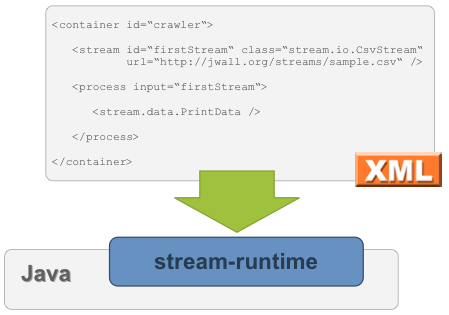
\includegraphics[scale=0.3]{graphics/quickstart-xml}
  \caption{\label{fig:quickstart}Conceptual way of executing a data flow graph that is defined in XML.}
\end{figure}

The simple example presented below, defines a single process that
reads from a CSV stream and prints out the data items to standard
output:

\begin{figure}[h!]
  \centering
  \begin{lstlisting}[language=XML]
    <container>
        <stream id="firstStream" class="stream.io.CsvStream"
                url="http://www.jwall.org/streams/sample-stream.csv" />

        <process input="firstStream">
            <PrintData />
        </process>
     </container>
  \end{lstlisting}
\end{figure}

The {\em stream-runner} required to execute this stream is a simple executable
Java archive available for download:
\begin{displaymath}
  \mbox{\url{http://download.jwall.org/streams/stream-runner.jar}}
\end{displaymath}


\subsubsection{Running a \streams Process}
The simple process defined above can be run by

\hspace{4ex}\sample{\# java -jar stream-runner.jar first-process.xml}

The process will simply read the stream in CSV-format and execute the
processor {\ttfamily PrintData} for each item obtained from the
stream.

\subsubsection{Including additional Libraries}
There exists a set pre-packaged libraries such as {\em streams-analysis}
or {\em streams-video}, which are provided at
\begin{displaymath}
  \mbox{\url{http://download.jwall.org/streams/libs/}}
\end{displaymath}
These add additional processors and stream implementations to the
\streams runtime for different domain specific intentions. To start
the \streams runtime with additional libraries, these need to be
provided on the classpath.

The following example uses the {\ttfamily MJpegImageStream} to process
a stream of video data from some URL. This stream implementation is
provided in the {\em streams-video} package.
\begin{figure}[h!]
  \centering
  \begin{lstlisting}[language=XML]
    <container>
        <stream id="video"
             class="stream.io.MJpegImageStream"
               url="http://download.jwall.org/streams/coffee.mjpeg.gz" />

        <process input="video" >

            <stream.image.DisplayImage key="data" />
            <stream.image.AverageRGB />

            <WithKeys keys="frame:*">
                 <stream.plotter.Plotter
       		         history="1000"
	                keepOpen="true"
	                keys="frame:red:avg,frame:green:avg,frame:blue:avg" />
            </WithKeys>
        </process>
    </container>
  \end{lstlisting}
  \caption{\label{fig:videoExample}Displaying an MJPEG video stream and plotting the average RGB channels.}
\end{figure}

For the libraries to be included in the path, the following command needs
to be issued to start the \streams run-time:

\hspace{4ex}\sample{\# java -cp stream-runner.jar:streams-video-0.0.1.jar $\backslash$
          stream.run video.xml}
